\documentclass[a4paper, 12pt]{article}

%\usepackage{cmap}
\usepackage[T2A]{fontenc}
\usepackage[utf8]{inputenc}
\usepackage[english, russian]{babel}
\usepackage{graphicx}
\usepackage[top=1in, bottom=1in, left=3.2cm, right=2.6cm]{geometry}
\graphicspath{./}
\usepackage{biblatex}
\addbibresource{lib.bib}
\linespread{1.5}

\usepackage{listings}
\usepackage{color}


\begin{document}
	
\begin{titlepage}
	\fontsize{12pt}{12pt}\selectfont
	\begin{figure}[t!]
		\centering
		
\includegraphics[scale=0.8]{bmstu}
	\end{figure}
	
	\noindent\rule{15cm}{3pt}
	\newline\newline
	\noindent 
	ФАКУЛЬТЕТ 
	\underline{«Информатика и системы управления»} \newline\newline
	
	\noindent КАФЕДРА \underline{«Программное обеспечение ЭВМ и информационные технологии»}\newline\newline\newline\newline\newline\newline
	
	\centering {\LARGE Отчет по лабораторной работе № 2}
	\vspace{3mm}
	
	\centering {\LARGE По курсу "Анализ Алгоритмов"
		\vspace{10mm}	
		
		\centering \bf Алгоритмы умножения матриц}
	\vspace{10mm}
	
	
	\begin{flushright}
		{\large	Студент:\\ Турсунов Жасурбек Рустамович \\ Группа: ИУ7-56Б
			\vspace{5mm}
			\\Преподователи: \\ Волкова Лилия Леонидовна \\ Строганов Юрий Владимирович}
	\end{flushright}
	
	\begin{center}
		\vfill
		Москва, \the\year
		~г.
	\end{center}
\end{titlepage}

\tableofcontents
\clearpage
\newpage

\section*{Введение}

\begin{flushleft}
	\hspace*{5mm} Целью данной лабораторной работы является изучение алгоритмов умножения матриц. В данной лабораторной работе рассматривается стандартный алгоритм умножения матриц, алгоритм Винограда и модифицированный алгоритм Винограда. Также требуется изучить рассчет сложности алгоритмов, получить навыки в улучшении алгоритмов. 
	\newline \hspace*{5mm} В ходе лабораторной предстоит выполнить следующие задачи: 
	\begin{enumerate}
		\item изучить алгоритмы умножения матриц; стандартный и алгоритм Винограда;
		\item оптимизировать алгоритм Винограда;
		\item дать теоретическую оценку базового алгоритма умножения матриц, алгоритма Винограда и улучшенного алгоритма Винограда;
		\item реализовать три алгоритма умножения матриц на одном из языков программирования;
		\item сравнить алгоритмы умножения матриц.
    \end{enumerate}
		
\end{flushleft}
\clearpage
\newpage
\section{Аналитическая часть}
\begin{flushleft}
	\hspace*{5mm} Матрицей А размера [m * n] называется прямоугольная таблица чисел, функций или алгебраических выражений, содержащая m строк и n столбцов. Числа m и n определяют размер матрицы. Если число столбцов в первой матрицы совпадает с числом строк во второй матрице, то эти матрицы можно перемножить. У произведения будет столько же строк, сколько в первой матрице и столько же столбцов, сколько во второй.
	\\ \hspace*{5mm} Пусть даны две прямоугольные матрицы A и B размеров [m * n] и [n * k] соответственно. В результате произведения матриц А и В получим матрицу C размера [m * k].\cite{mul}
	\begin{figure}[h]
		\hspace{5mm}
		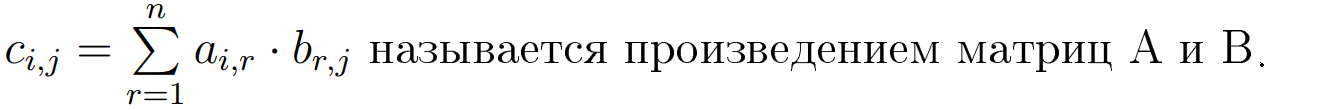
\includegraphics[scale=0.8]{formula1}
	\end{figure} 
	\subsection{Алгоритм Винограда}
	\hspace*{5mm} Подход Алгоритма Винограда является иллюстрацией общей методологии, начатой в 1979-ч годах на основе билинейных и трилинейных форм, благодоря которым большинство усовершенствований для умножения матриц были получены с помощью разложения скалярного произведения векторов. {\it v}1
	\\ \hspace*{5mm} Рассмотрим два вектора {\it V} = ({\it v}1, {\it v}2, {\it v}3, {\it v}4) и {\it W} = ({\it w}1, {\it w}2, {\it w}3, {\it w}4). 
	\\ \hspace*{5mm} Их скалярное произведение равно (1.1)
	\begin{figure}[h]
		\centering
		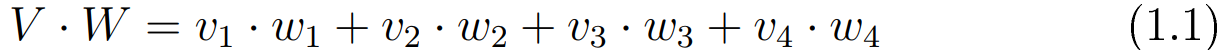
\includegraphics[scale=0.8]{formula2}
	\end{figure}
	\\ \hspace*{5mm} Равенство (1.1) можно переписать в виде (1.2)
	\begin{figure}[h]
		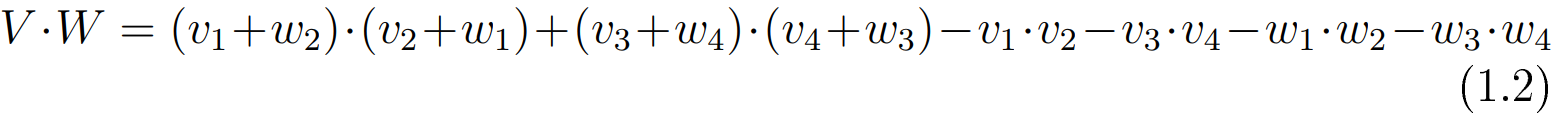
\includegraphics[scale=0.8]{formula3}
	\end{figure}
	\\ \hspace*{5mm} Менее очевидно, что выражение в правой части последнего равенства допускает предварительную обработку: его части можно вычислить заранее и запомнить для каждой строки первой матрицы и для каждого столбца второй. Это означает, что над предварительно обработанными элементами нам придется выполнить лишь первые два умножения и последующие пять сложений, а также дополнительно два сложения.
	\subsection{Вывод}
	\hspace*{5mm} Были рассмотрены алгоритмы классического умножения матриц и алгоритм Винограда.\cite{mulAlg} \\Главное отличие которых - наличие предварительной обработки, а также количество операций умножения.
\end{flushleft}

\newpage
\section{Конструкторская часть}
\begin{flushleft}
	{\bf Требования к вводу: } На вход подаются две матрицы.
	\begin{enumerate}
		\item на вход подаются две строки;
		\item строчные и заглавные буквы считаются разными;
	\end{enumerate}
		{\bf Требования к программе: } На вход подаются две матрицы.
	\begin{enumerate}
		\item корректное умножение двух матриц;
		\item при матрицах разных размеров программа не должнв аварийно завершаться. 
	\end{enumerate}

	\subsection{Разработка алгоритмов}
	В данном разделе будут рассмотрены схемы алгоритмов:
	\begin{enumerate}
		\item классический алгоритм умножения матриц;
		\item алгоритм Винограда;
		\item оптимизированный алгоритм Винограда.
	\end{enumerate}
	\clearpage
	\newpage
	\hspace*{5mm} На рисунке 1 представлена схема классического алгоритма умножения матриц.
	\begin{figure}[h!]
		\centering 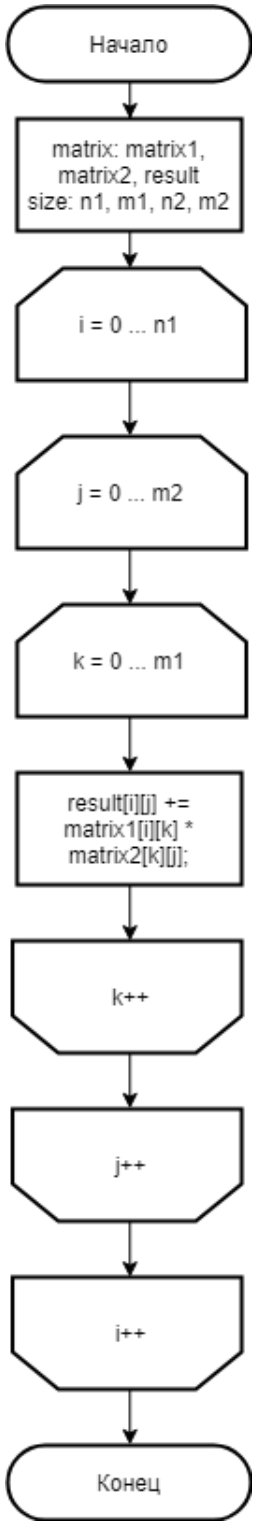
\includegraphics[scale=1.2]{classic}
		\centering \caption{Схема классического алгоритма умножения матриц}
	\end{figure}
	\clearpage
	\newpage
	\hspace*{5mm} На рисунке 2 представлена схема алгоритма Винограда.
	\begin{figure}[h!]
		\centering 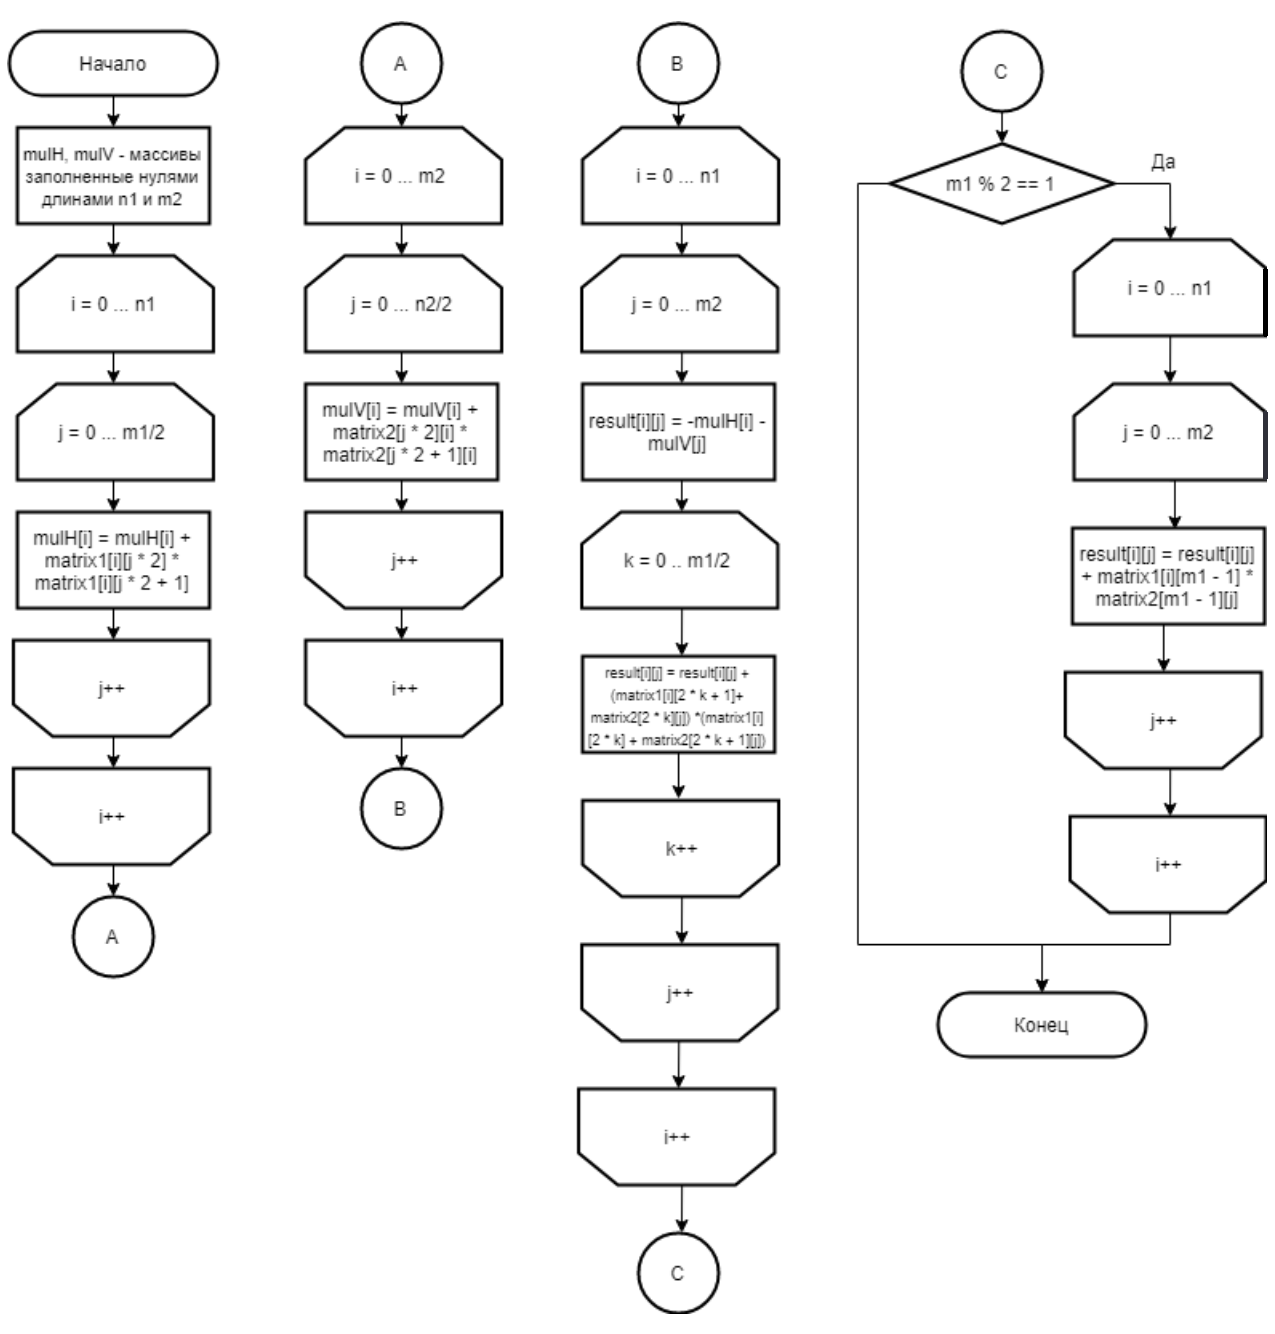
\includegraphics[scale=1.3]{vinograd}
		\centering \caption{Схема алгоритма Винограда}
	\end{figure}
    \clearpage
	\newpage
	\hspace*{5mm} На рисунке 3 представлена схема оптимизированного алгоритма Винограда.
	\begin{figure}[h!]
		\centering 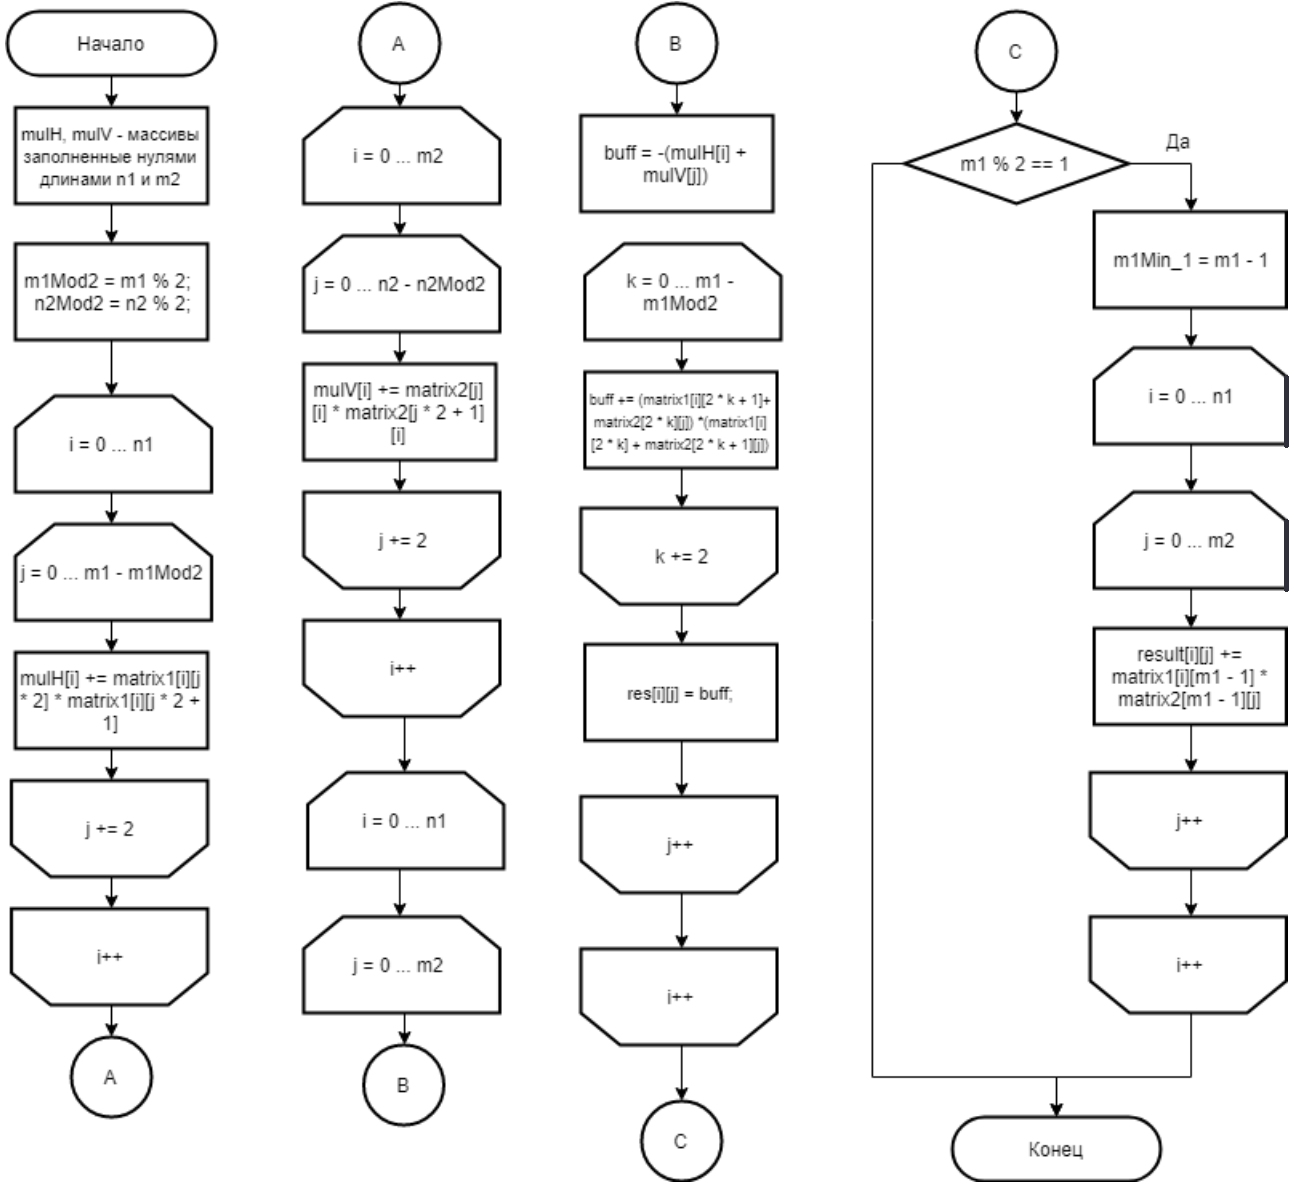
\includegraphics[scale=1.3]{optimizedvinograd}
		\centering \caption{Схема оптимизированного алгоритма Винограда}
	\end{figure}
	\clearpage
	\newpage
	\subsection{Трудоемкость алгоритмов}
	Введем модель трудоемкости для оценки алгоритмов:
	\begin{enumerate}
		\item базовые операции стоимостью 1 - +, -, *, /, =, ==, <=, >=, !=, +=, [], получение полей класса;
		\item оценка трудоемкости цикла: Fц = init + N * (a + Fтела + post) + a, \\где а - условие цикла, init - предусловие цикла, post - постусловие цикла;
		\item стоимость условного перехода применим за 0, стоимомть вычисления условия остаётся. 
	\end{enumerate}
	Оценим трудоемкость алгоритмов по коду программы.
	\subsubsection{Классический алгоритм}
	Рассмотрим трудоемкость первичной проверки на возможность умножения матриц.
	\\ \hspace*{5mm} Инициализация матрицы результата: 1 + 1 + {\it n}$_1$(1 + 2 + 1) + 1 = 4{\it n}$_1$ + 3.
	\\ \hspace*{5mm} Подсчёт:
	\\ 1 + {\it n}$_1$(1 + (1 + {\it m}$_2$(1 + (1 + {\it m}$_1$(1 + (8) + 1) + 1) + 1) + 1) + 1) + 1 =
	{\it n}$_1$({\it m}$_2$(10{\it m}$_1$ + 4) + 4) + 4) + 2 = 10{\it n}$_1${\it m}$_2${\it m}$_1$ + 4{\it n}$_1${\it m}$_2$ + 4{\it n}$_1$ + 2.
	
	\subsubsection{Алгоритм Винограда}
	\begin{figure}[h]
		\centering 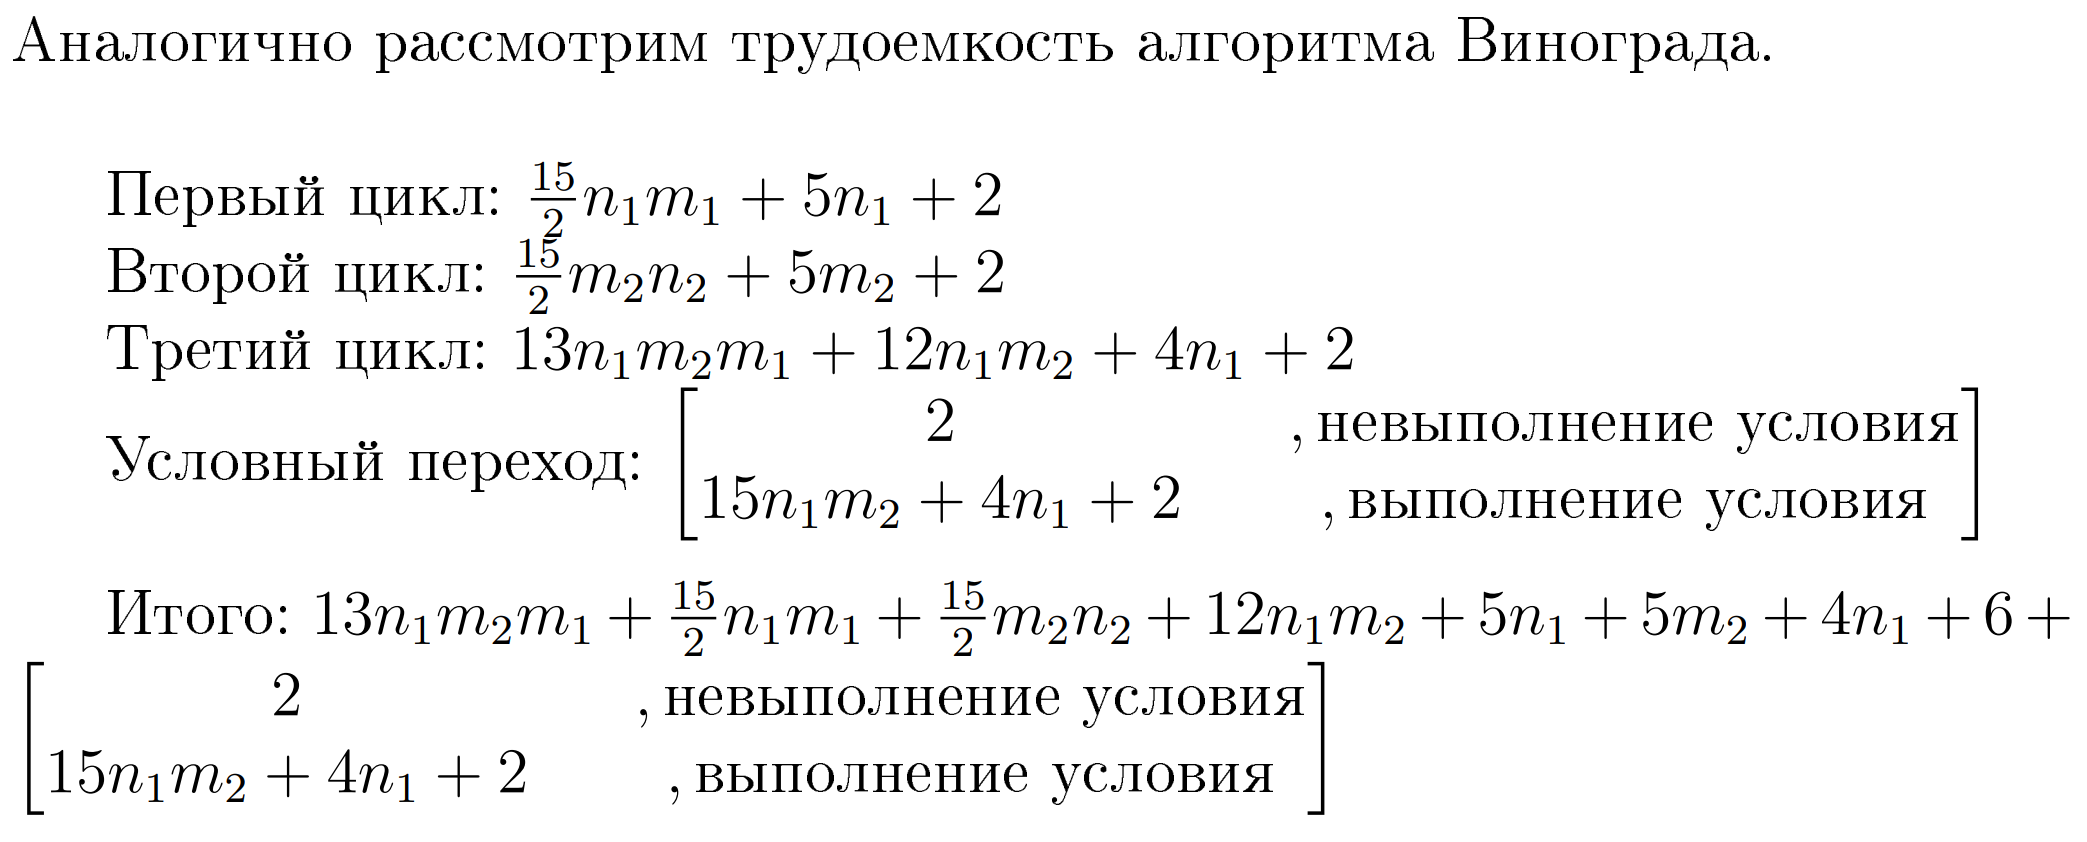
\includegraphics[scale=0.65]{223}
	\end{figure}
	\clearpage
	\newpage
	\subsubsection{Оптимизированный алгоритм Винограда}
	\begin{figure}[h]
		\centering 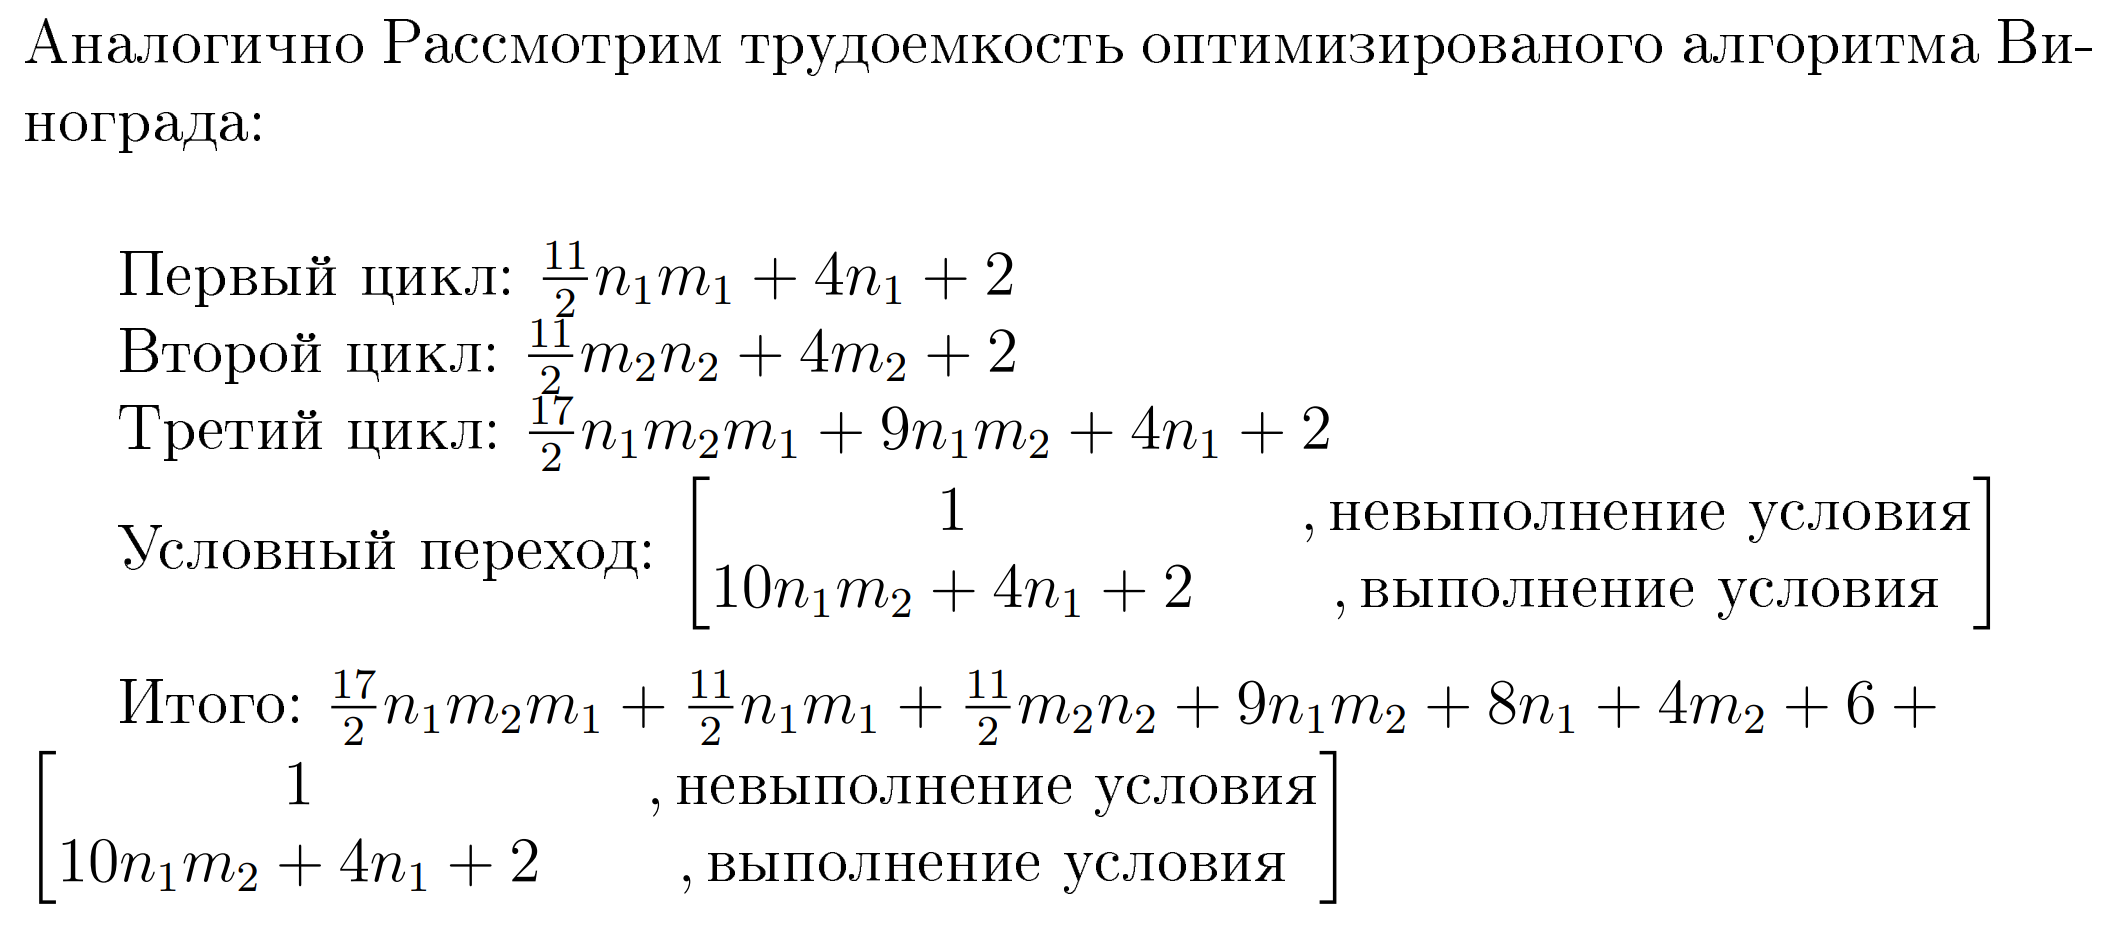
\includegraphics[scale=0.65]{224}
	\end{figure}
	\subsection{Вывод}
	\hspace*{5mm} В данном разделе были рассмотрены схемы алгоритмов умножения матриц, введена модель оценки трудоемкости алгоритма, были расчитаны трудоемкости алгоритмов в соответствии с этой моделью.
\end{flushleft}

\newpage
\section{Технологическая часть}
\begin{flushleft}
	\hspace*{5mm} В данном разделе будут рассмотрены требования к программному обеспечению, средства реализации и представлен листинг кода.
	\subsection{Требования к программному обеспечению}
	\hspace*{5mm} Входные данные: две матрицы.
	\\ \hspace*{5mm} Выходные данные: матрица полученная в результате умножения двух матриц.
	\\ \hspace*{5mm} На рисунке 4 представлена IDEF0-диаграмма, описывающая функциональную схему умножения матриц.
	\begin{figure}[h!]
		\centering 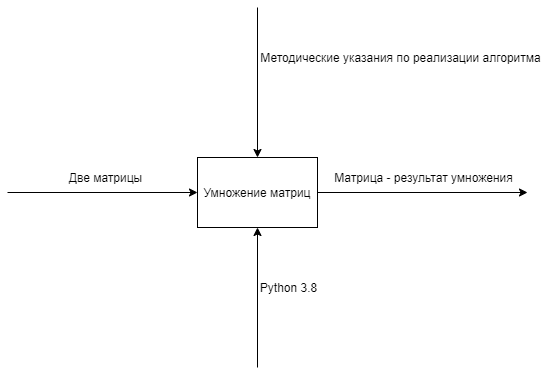
\includegraphics[scale=0.8]{диаграмма}
		\centering\caption{IDEF0-диаграмма, описывающая функциональную схему умножения матриц.}
	\end{figure}
	\clearpage
	\newpage
	\subsection{Средства реализации}
	\hspace*{5mm} В данной работе используется язык программирования Python, так как ЯП позволяет написать программу за кратчайшее время. Проект выполнен в среде разработки Visual Studio Code.
	\subsection{Листинг кода}
	В данном пункте представлен листинг кода, а именно:
	\begin{itemize}
		\item классический алгоритм умножения матриц;
		\item алгоритм Винограда;
		\item оптимизированный алгоритм Винограда.
	\end{itemize}
	\definecolor{codegreen}{rgb}{0,0.6,0}
	\definecolor{codegray}{rgb}{0.5,0.5,0.5}
	\definecolor{codepurple}{rgb}{0.58,0,0.82}
	\definecolor{backcolour}{rgb}{0.95,0.95,0.92}

	\lstdefinestyle{mystyle}{
		backgroundcolor=\color{backcolour},   
		commentstyle=\color{codegreen},
		keywordstyle=\color{magenta},
		numberstyle=\tiny\color{codegray},
		stringstyle=\color{codepurple},
		basicstyle=\ttfamily\footnotesize,
		breakatwhitespace=false,         
		breaklines=false,                 
		captionpos=b,                    
		keepspaces=true,                 
		numbers=left,                    
		numbersep=5pt,                  
		showspaces=false,                
		showstringspaces=false,
		showtabs=false,                  
		tabsize=4
	}

	\lstset{style=mystyle}

	\hspace*{5mm} На листинге 1 представлен код классического алгоритма умножения матриц.
	\begin{lstlisting}[language=Python, caption = Классический алгоритм умножения матриц]
	def classicMul(a, b):
		if len(b) != len(a[0]):
			print("Different dimension of the matrics")
			return
		n = len(a)
		m = len(a[0])
		k = len(b[0])
		res = [[0 for i in range(0, k)] for j in range(0, n)]
		for i in range(n):
			for j in range(m):
				for t in range(k):
					res[i][t] += a[i][j] * b[j][t]
		return res
	\end{lstlisting}
	\clearpage
	\newpage
	\hspace*{5mm} На листинге 2 представлен код алгоритма Винограда.
	\begin{lstlisting}[language=Python, caption = Алгоритм Винограда]
		def classicVinograd(G, H):
			a = len(G)
			b = len(H)
			c = len(H[0])
			if b != len(G[0]):
				print("Different dimension of the matrics")
				return
			d = b // 2
			row = [0 for i in range(a)]
			col = [0 for i in range(c)]
			for i in range(a):
				for j in range(d):
					row[i] += G[i][2 * j] * G[i][2 * j + 1]
			for i in range(c):
				for j in range(d):
					col[i] += H[2 * j][i] * H[2 * j + 1][i]
		
			answer = [[0 for i in range(c)] for j in range(a)]
			for i in range(a):
				for j in range(c):
					answer[i][j] = - row[i] - col[j]
					for k in range(d):
						answer[i][j]+=((G[i][2*k] + 
								H[2*k+1][j])*(G[i][2*k+1]+H[2*k][j]))
			if b % 2:
				for i in range(a):
					for j in range(c):
						answer[i][j] += G[i][b - 1] * H[b - 1][j]
		
			return answer
	\end{lstlisting}
	\clearpage
	\newpage
	\hspace*{5mm} На листинге 3 представлен код оптимизированного алгоритма Винограда.
	\begin{lstlisting}[language=Python, caption = Оптимизированный алгоритм Винограда]
		def imprvVinograd(G, H):
		a = len(G)
		b = len(H)
		c = len(H[0])
		
		if b != len(G[0]):
			print("Different dimension of the matrics")
			return
		
		d = b // 2
		
		row = [0 for i in range(a)]
		col = [0 for i in range(c)]
		
		for i in range(a):
			row[i]=sum(G[i][2*j]*G[i][2*j+1] for j in range(d))
		
		for i in range(c):
			col[i]=sum(H[2*j][i]*H[2*j+1][i] for j in range(d))
		
		answer = [[0 for i in range(c)] for j in range(a)]
		for i in range(a):
			for j in range(c):
				answer[i][j]=sum((G[i][2 k]+H[2*k+1][j])*
				   (G[i][2*k+1]+H[2*k][j]) for k in range(d))
				   						-row[i]-col[j]
	
		if b % 2:
			for i in range(a):
			  answer[i][j]=sum(G[i][b-1]*H[b-1][j] for j in range(c))
	
		return answer
	\end{lstlisting}
	\subsection{Вывод}
	\hspace*{5mm} В данном разделе была представлена структура ПО и листинги кода программы. 
	
\end{flushleft}

\newpage
\section{Исследовательская часть }
\begin{flushleft}
	\hspace*{5mm} В данном разделе будет проведен эксперимент и сравнительный анализ.
	\subsection{Системные характеристики}
	Характеристики компьютера на котором проводился замер времени сортировки массива:
	\begin{enumerate}
		\item операционная система - Windows 10;
		\item процессор - Intel(R) Core(TM) i7-10510U CPU @1.80GHz 2.30GHz;
		\item оперативная память - 16 ГБ.
	\end{enumerate}
	\subsection{Постановка эксперимента}
	В рамках данного проекта были проведены эксперименты, описанные ниже:
	\begin{enumerate}
		\item Сравнение времени работы алгоритмов при четном и нечеином размере матрицы.
	\end{enumerate}
	\subsection{Сравнительный анализ на основе замеров времени работы алгоритмов}
	Был проведен замер времени работы каждого из алгоритмов.
	\\ \hspace*{5mm} На рисунке 5 показаны результаты первого эксперимента, который производится для лучшего случая на квадратных матрицах размером от 100 х 100 до 1000 х 1000 с шагом 100. Ниже приведена полученная диаграмма:
	\clearpage
	\newpage
	\begin{figure}[h]
		\centering 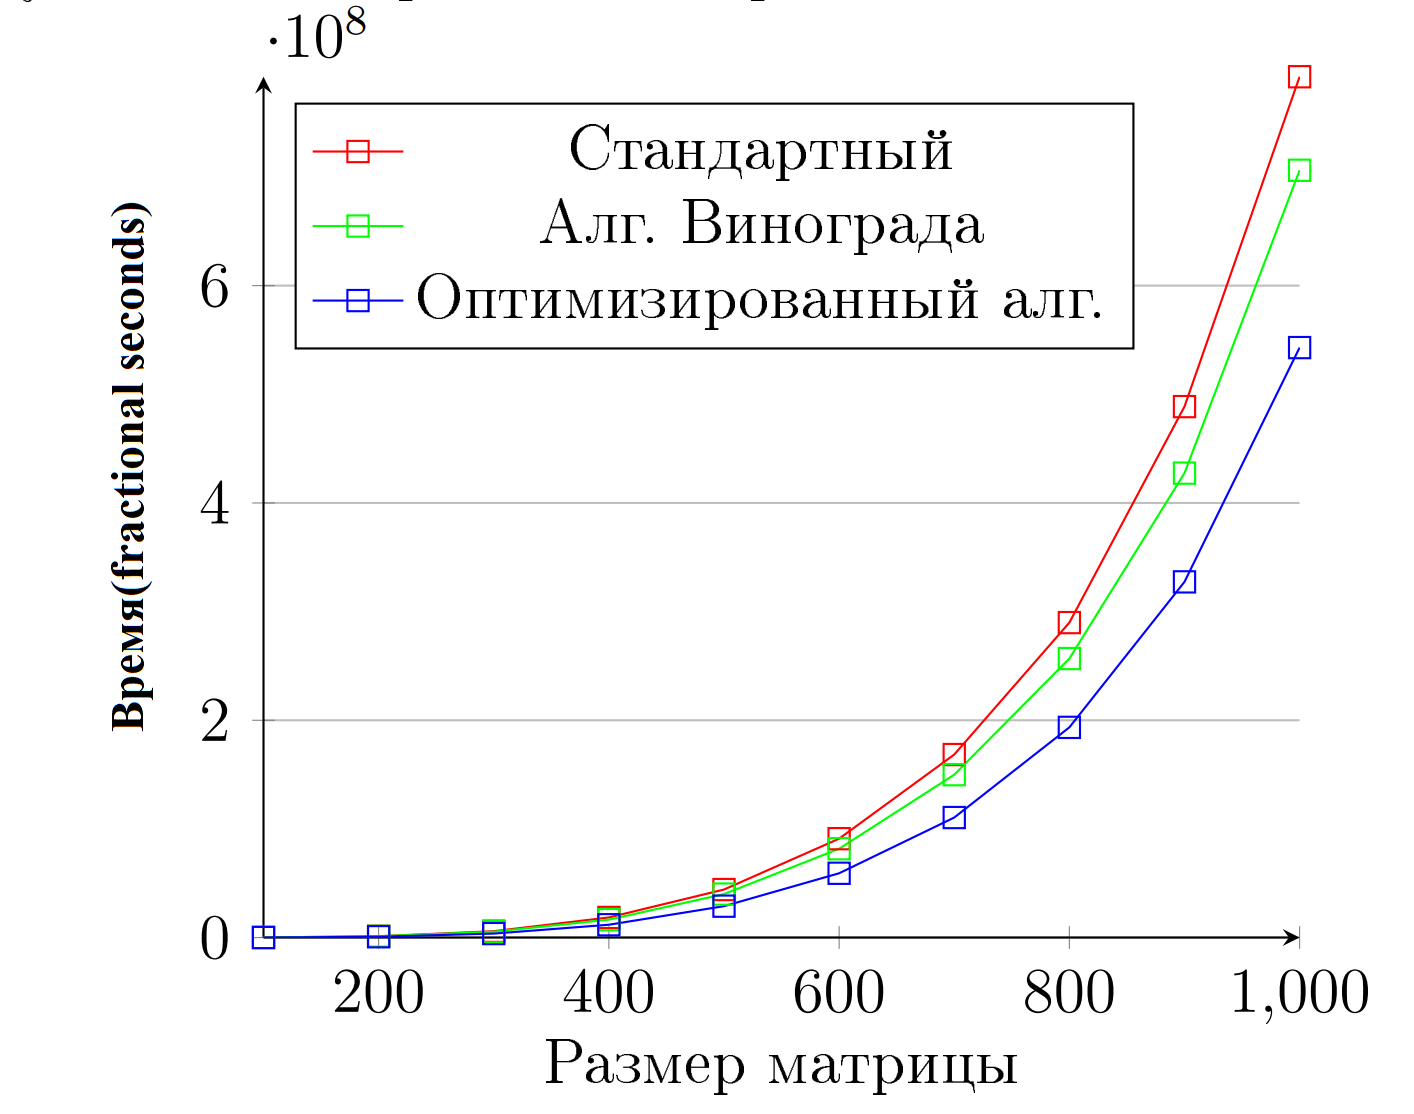
\includegraphics[scale=0.85]{time1}
		\centering\caption{Сравнение времени работы алгоритмов при четном размере матрицы}
	\end{figure}
	
	\hspace*{5mm} На рисунке 6 показаны результаты второго эксперимента, который производится для худшего случая, когда поданы квадратные матрицы с нечетными размерами от 101 х 101 до 1001 х 1001 с шагом 100. Ниже приведена полученная диаграмма:
	\clearpage
	\newpage 
	\begin{figure}[h]
		\centering 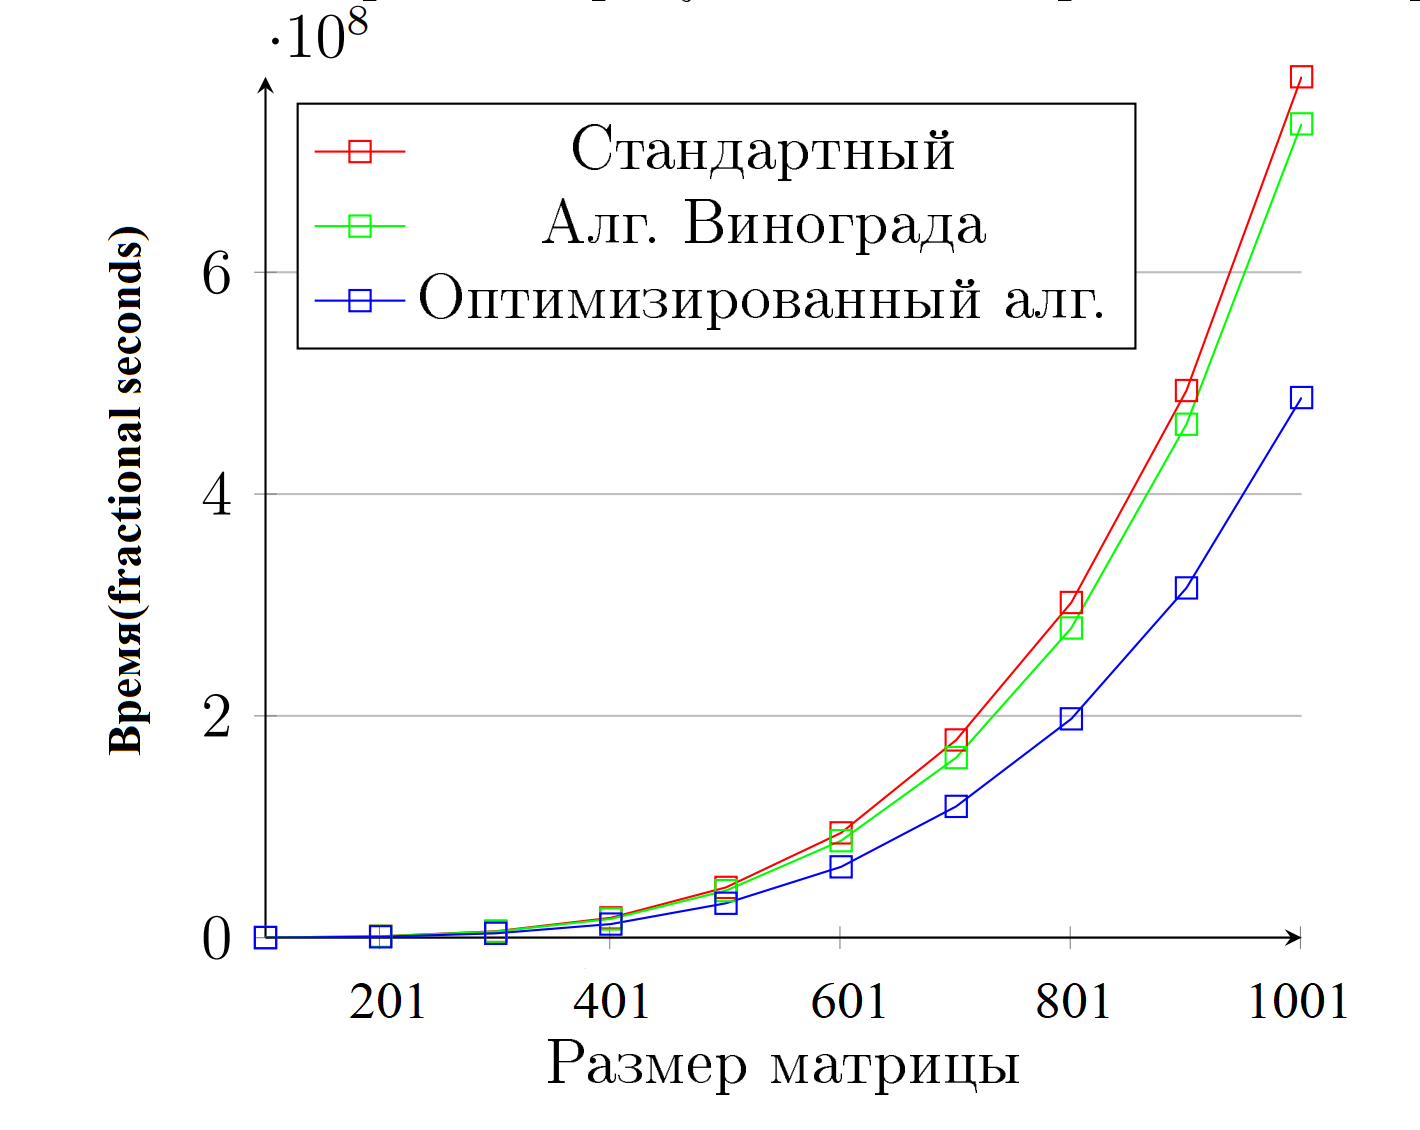
\includegraphics[scale=0.9]{time2}
		\centering\caption{Сравнение времени работы алгоритмов при нечетном размере матрицы}
	\end{figure}
	\clearpage
	\newpage
	\subsection{Тестирование программы}
	В данном разделе будут показаны результаты тестирования
	\\ \hspace*{5mm} Всего было реализовано 7 тестовых случаев:
	\begin{enumerate}
		\item Некорректный размер матриц;
		\item Размер матрицы равен 1;
		\item Размер матрицы равен 2; 
		\item Сравнение работы стандартной реализации с алгоритмом Винограда на случайных значениях при четном и нечетном размерах матриц;
		\item Сравнение работы стандартной реализации с оптимизированным алгоритмом Винограда на случайных значениях при четном и нечетном размерах матриц;
	\end{enumerate}
	\hspace*{5mm} На рисунке 7 показаны результаты тестирования
	\begin{figure}[h]
		\centering 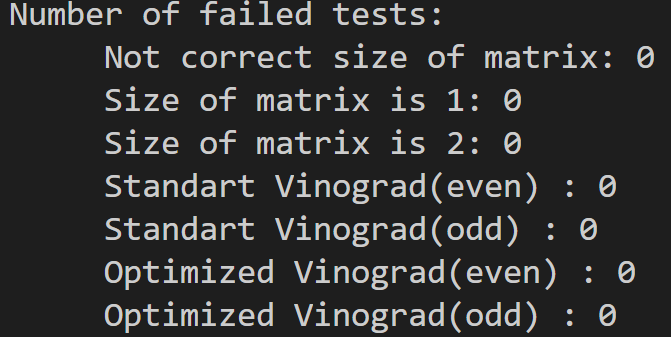
\includegraphics[scale=1.2]{tests}
		\centering\caption{Результаты тестирования}
	\end{figure}
	\subsection{Вывод}
	\hspace*{5mm} По результатам тестирования все рассматриваемые алгоритмы были реализованы верно. Самым медленным алгоритмом оказался алгоритм классического умножения матриц, а самым быстрым - оптимизированный алгоритм Винограда.
\end{flushleft}

\begin{flushleft}
	\newpage
	\section*{Заключение}
	\hspace*{5mm} В ходе работы были изучены алгоритмы классического умножения матриц, стандартный и оптимизированный алгоритм Винограда. Также была дана теоретическая оценка алгоритмам умножения матриц. Было сделано сравнение этих алгоритмов, также был реализован программный код продукта.  
\end{flushleft}

\clearpage
\newpage

\printbibliography

\end{document}